\section{Реализация программного средства}

Реализация программного средства обнаружения аномалий в логах Kubernetes выполнена в виде многомодульного приложения, построенного по принципам чистой архитектуры. Такой подход позволяет разделить ответственность между компонентами системы, повысить её расширяемость и упростить сопровождение.

Программное средство состоит из следующих основных компонентов:

\begin{itemize}
    \item серверное приложение (backend);
    \item процесс фоновой обработки задач (worker);
    \item клиентский веб-интерфейс (frontend);
    \item инфраструктурные компоненты (база данных, очередь задач, хранилище логов).
\end{itemize}

Логическая структура приложения организована в виде слоёв:

\begin{itemize}
    \item слой представления (frontend);
    \item слой API;
    \item прикладной слой (business logic);
    \item доменный слой;
    \item инфраструктурный слой.
\end{itemize}

Общая структура зависимостей модулей серверного приложения представлена на рисунке~\ref{fig:uml_master}.

\begin{figure}[H]
    \centering
    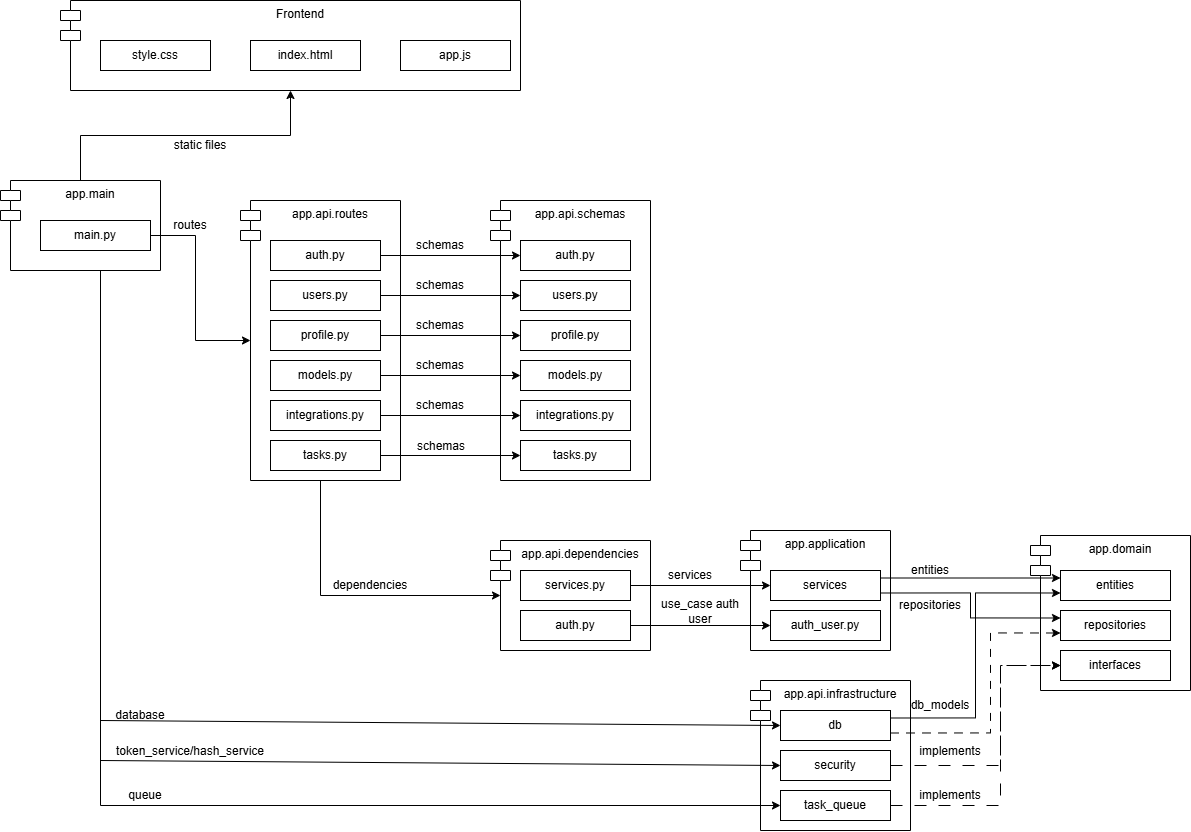
\includegraphics[scale=0.3]{inc/images/uml_master}
    \caption{UML-диаграмма зависимостей модулей основного приложения}
    \label{fig:uml_master}
\end{figure}

Общая структура зависимостей модулей процесса фоновой обработки задач представлена на рисунке~\ref{fig:uml_worker}.

\begin{figure}[H]
    \centering
    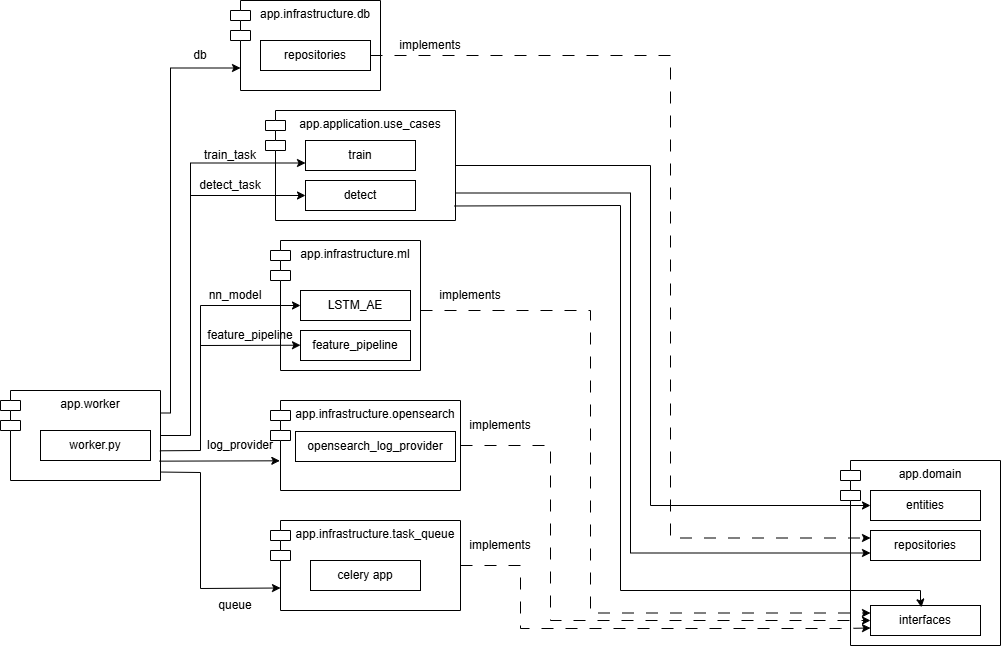
\includegraphics[scale=0.3]{inc/images/uml_worker}
    \caption{UML-диаграмма зависимостей процесса фоновой обработки}
    \label{fig:uml_worker}
\end{figure}

Основным модулем системы является файл \texttt{main.py}, который выполняет инициализацию веб-приложения. В данном модуле создаётся экземпляр FastAPI-приложения, подключаются маршруты API, настраивается обработка ошибок, а также конфигурируются внешние зависимости, включая подключение к базе данных, систему аутентификации и очередь задач. Кроме того, данный модуль отвечает за раздачу статических файлов пользовательского интерфейса и настройку CORS, что обеспечивает корректное взаимодействие между клиентской и серверной частями.


Модули, расположенные в директории \texttt{app/api/routes/}, реализуют REST API приложения. Каждый модуль отвечает за отдельную функциональную область (аутентификация, управление пользователями, моделями, задачами и интеграциями). Маршруты принимают HTTP-запросы и передают их на обработку в прикладной слой.

Для описания структуры входных и выходных данных используются модули \texttt{app/api/schemas/}, реализующие схемы на основе Pydantic. Это обеспечивает строгую типизацию, валидацию данных и единый контракт взаимодействия с клиентом.

Прикладной слой представлен модулями \texttt{app/application/services/} и \texttt{app/application/use\_cases/}. Данный слой реализует бизнес-логику системы и сценарии использования. Сервисы инкапсулируют операции над сущностями предметной области, такими как пользователи, модели и задачи. Сценарии (\textit{use cases}) описывают конкретные процессы, включая:

\begin{itemize}
    \item постановку задачи обучения модели;
    \item запуск процесса детектирования аномалий;
    \item управление жизненным циклом задач.
\end{itemize}

Ключевыми компонентами являются модули \texttt{train.py} и \texttt{detect.py}, реализующие обучение и применение моделей на основе LSTM-AE.

Модуль \texttt{worker.py} реализует отдельный процесс обработки фоновых задач с использованием Celery. Он выполняет ресурсоёмкие операции, такие как обучение моделей и анализ логов, вне основного HTTP-потока. Такое разделение позволяет повысить отзывчивость системы и обеспечить масштабируемость за счёт распределённого выполнения задач.

Доменный слой содержит описание сущностей предметной области, интерфейсов репозиториев и абстракций, используемых в системе. Он не зависит от конкретных технологий хранения данных или реализации моделей, что обеспечивает независимость бизнес-логики от инфраструктуры.

Инфраструктурный слой включает реализацию взаимодействия с внешними системами:

\begin{itemize}
    \item модуль работы с базой данных (\texttt{PostgreSQL});
    \item модуль взаимодействия с OpenSearch для получения audit-логов;
    \item модуль машинного обучения (реализация LSTM-AE);
    \item модуль очереди задач (Celery, Redis);
    \item модуль безопасности (JWT-аутентификация).
\end{itemize}

Данный слой реализует интерфейсы, определённые в доменном слое, обеспечивая тем самым связанность компонентов системы.

Клиентская часть реализована в виде одностраничного приложения, включающего файлы:

\begin{itemize}
    \item \texttt{index.html} — структура интерфейса;
    \item \texttt{style.css} — оформление;
    \item \texttt{app.js} — логика взаимодействия с API.
\end{itemize}

Взаимодействие с сервером осуществляется посредством REST API. Клиентская логика обеспечивает отправку запросов, получение результатов и их визуализацию.

\subsection{Взаимодействие модулей}

Взаимодействие компонентов системы организовано следующим образом:

\begin{enumerate}
    \item Пользователь взаимодействует с веб-интерфейсом, который формирует HTTP-запросы к серверу.
    \item Запрос поступает в модуль маршрутов FastAPI, где происходит его валидация и передача в прикладной слой.
    \item Прикладной слой инициирует выполнение соответствующего сценария, который может включать обращение к базе данных или постановку задачи в очередь.
    \item В случае длительных операций (обучение модели или детектирование) создаётся задача в очереди Celery.
    \item Процесс \texttt{worker.py} извлекает задачу из очереди, выполняет обработку данных, взаимодействует с OpenSearch и сохраняет результаты в базу данных.
    \item Клиент периодически запрашивает статус задачи и получает результаты через API.
\end{enumerate}

Таким образом, система реализует асинхронную модель взаимодействия, позволяющую эффективно обрабатывать большие объёмы данных и обеспечивать масштабируемость при увеличении нагрузки.